\documentclass[12pt, a4paper, oneside, british]{report}
\usepackage{epigraph}
\usepackage{setspace}
\usepackage{gensymb}
\usepackage[dvipsnames]{xcolor}
\usepackage[british]{babel}
\usepackage{amssymb}
\usepackage{amsmath}
\usepackage{pgfplotstable}
\usepackage{pgfplots}
\usepackage{natbib}
\usepackage[hyphens]{url}


\usepackage{multicol}
\usepackage{blindtext}

\bibliographystyle{abbrvnat}

%Diagramme
\usepackage{pgfplots}
\usepackage{pgfplotstable}

\usepackage[singlelinecheck=false,font={footnotesize, it}, tablewithin=section,
figurewithin=section,format=hang]{caption}

\usepackage{multirow}
\usepackage{footnote}
\makesavenoteenv{tabular}
%To Use Float Barrier
\usepackage{placeins}

%For Listings
\usepackage{listings}
\usepackage{lstlinebgrd}


%For Abbreviations
\usepackage[printonlyused]{acronym}

%For Headers and Footers
\usepackage{fancyhdr}
\pagestyle{fancy}
\fancyhf{}

\lfoot{TSMW - Interim Report}
\rfoot{17\textsuperscript{th} April 2017}
\renewcommand{\headrulewidth}{1pt}
\renewcommand{\footrulewidth}{1pt}


\makeatletter
% we use \prefix@<level> only if it is defined
\renewcommand{\@seccntformat}[1]{%
  \ifcsname prefix@#1\endcsname
    \csname prefix@#1\endcsname
  \else
    \csname the#1\endcsname\quad
  \fi}
% define \prefix@section
\newcommand\prefix@section{ }
\newcommand\prefix@subsection{ }
\makeatother

\setlength\columnsep{30pt}

\begin{document}
%\onehalfspacing
\begin{center}

\includegraphics[width=0.3\textwidth]{logo.png}

\vspace{0.5cm}

{\Large
\textbf{TSMW}}
\end{center}

\begin{multicols}{2}[\section{Interim Report on the Project's Progress}]
Dear Customer,

\vspace{0.5cm}
\noindent we'd like to present you the information about our current progress. Please let us know if there are any questions or remarks on the recently made decisions or on the progress itself.

\subsection{Recent Activities}
The recently completed activities include:
\begin{itemize}
\item Refinement of the Scope according to our most recent agreements (see the email, 7\textsuperscript{th} April, 2017)
\item Refinement of the final Requirements according to you feedback
\item Finalisation of the market analysis regarding the competitors on the market as well as regarding the available hardware parts
\item Finalisation of System Analysis including the gained knowledge from your last feedback form
\item Finalisation of the needed algorithms' analysis
\item Creation of improved skins for day- and night-mode
\item Implementation of the data storage 
\end{itemize}

\subsection{Current Timeplan}
Unfortunately, as you were informed by the email of the 13\textsuperscript{th} April 2017, we ran into some problems regarding the implementation of the data storage. These problems, causing an initial delay of 3 days on this tasks, could now be overcome. Since the implementation of the depending systems could nevertheless be continued with only little overhead of abstracting the real data storage, the total delay is currently only about one day and will be compensable by time buffer we included in our project plan.

\subsection{Cost Estimation for a Hardware - PoC}
As you required, we made an estimation about the costs to create a Hardware-PoC. Please let us know if you are interested in the justification of the used components.

\vspace{0.25cm}
{\footnotesize
\renewcommand{\arraystretch}{1.5}
\begin{tabular}{ll}
Part & Costs \\
\hline
2x 32KM NTSC & \hspace{0.07cm} 63.90\$ \\
4x LV-MaxSonar-EZ1  & \hspace{0.07cm} 93.44\$ \\
1x Arduino Mega 2560 & \hspace{0.07cm} 37.18\$ \\ 
\hline
Total & 194.52\$
\end{tabular}}

\subsection{Final Results of the System Analysis}
The context of the system is depicted below. It shows you all the systems that we expect to get input from and all the components we plan to actuate. If you need further insights into the analysis we conducted, we will send you the complete analysis in a separate document.
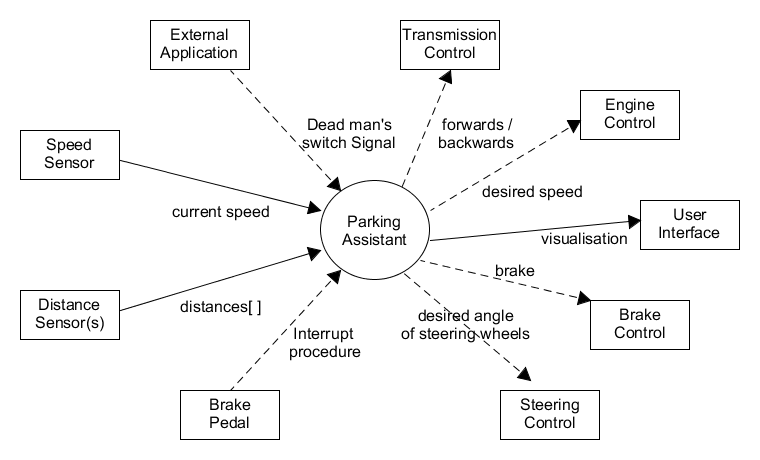
\includegraphics[width=0.45\textwidth]{ContextDiagram.png}

\subsection{Improved Skins}
According to your feedback, we improved the available skins of the system. In addition to the first presented skin, we created a brighter skin that might be used in the day-mode. We also included your feedback regarding the simplification of the outputs and extended the area where the relevant sensor information is represented.

\vspace{0.5cm}

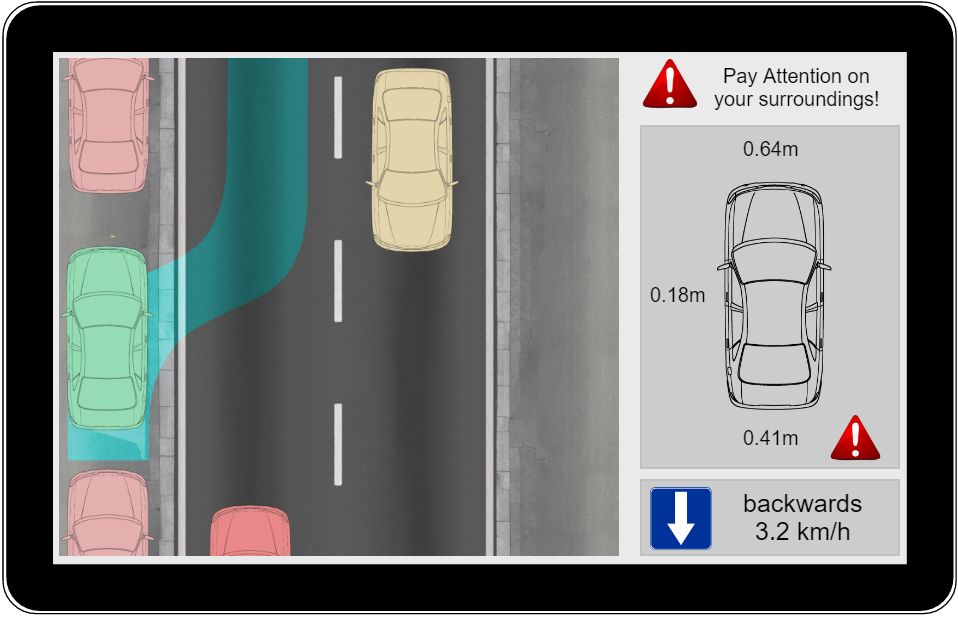
\includegraphics[width=0.45\textwidth]{brightskin.png}

\vspace{0.5cm}

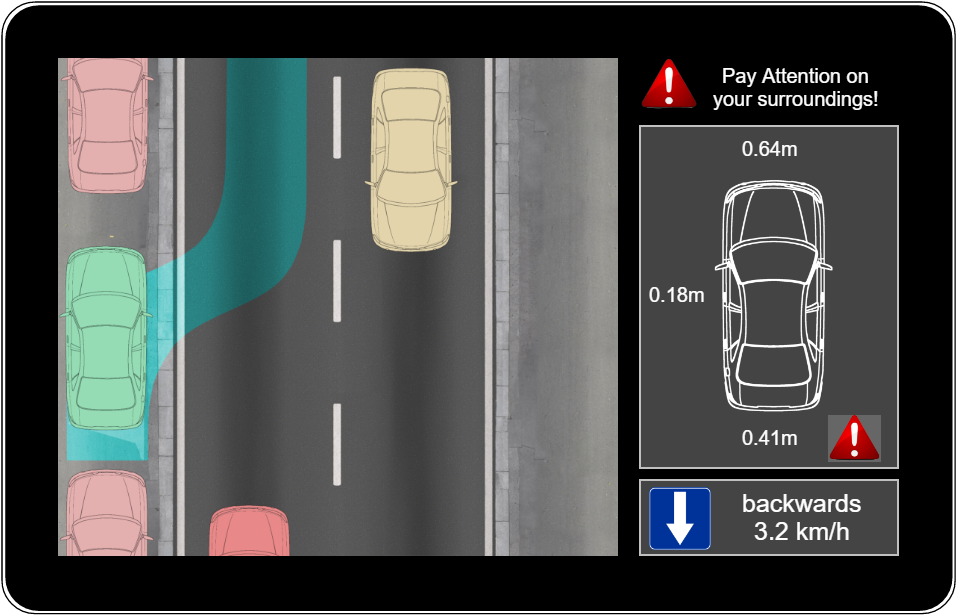
\includegraphics[width=0.45\textwidth]{darkskin.png}

\section{Next Steps}
Our next steps will be the final inclusion of the data storage as well as the enhancement of testing. In parallel, we will refine the current documentation and prepare the review / presentation of the developed product.


\end{multicols}


\end{document}
